%%%%%%%%%%%%%%%%%%%%%%%%%%%%%%%%%%%%%%%%%%%%%%%%%%
%% Bachelor's & Master's Thesis Template        %%
%% Copyleft by Dawid Weiss & Marta Szachniuk    %%
%% Faculty of Computing and Telecommunication   %%
%% Poznan University of Technology, 2020        %%
%%%%%%%%%%%%%%%%%%%%%%%%%%%%%%%%%%%%%%%%%%%%%%%%%%

% Szkielet dla pracy Magisterskiej pisanej w języku polskim.

\documentclass[polish,a4paper,oneside]{ppfcmthesis}
\pagenumbering{arabic}

\usepackage[utf8]{inputenc}
\usepackage[OT4]{fontenc}
\usepackage{float}
\usepackage[inkscapelatex=false]{svg}
\usepackage{geometry}
\usepackage{graphicx}
\usepackage{tocloft}
\usepackage{msc}
\usepackage{pgfplots}
\usepackage{tikz}
\pgfplotsset{compat=1.17}
\usepackage{listings}

% Define custom colors
\definecolor{comment}{rgb}{0.5,0.5,0.5}
\definecolor{keyword}{rgb}{0.0,0.0,0.8}
\definecolor{string}{rgb}{0.8,0.0,0.0}

% Define Java language settings for listings
\lstdefinestyle{customjava}{
  language=Java,
  basicstyle=\ttfamily\footnotesize,
  keywordstyle=\color{keyword}\bfseries,
  commentstyle=\color{comment}\itshape,
  stringstyle=\color{string},
  numberstyle=\tiny\color{comment},
  stepnumber=1,
  numbersep=10pt,
  showspaces=false,
  showstringspaces=false,
  tabsize=4,
  breaklines=true,
  breakatwhitespace=false,
  escapeinside={(*@}{@*)}
}

% Set the style for listings
\lstset{style=customjava}

%--------------------------------------
% Strona tytułowa
%--------------------------------------

% Autorzy pracy, jeśli jest ich więcej niż jeden
% wstaw między nimi separator \and
\author{% 
    Jan Biały \album{144334}}
\authortitle{inż.}

\title{Zarządzanie przydziałem zasobów w środowisku Metaverse}

% Your supervisor comes here.
\ppsupervisor{prof.~dr hab.~inż.~Anna Kobusińska} 

% Year of final submission (not graduation!)
\ppyear{2024}                                 

\begin{document}
\pagestyle{ppfcmthesis}%

% Front matter starts here
\pagestyle{empty}%
\maketitle\cleardoublepage%

%--------------------------------------
% Miejsce na kartę pracy dyplomowej
%--------------------------------------

\thispagestyle{empty}\vspace*{\fill}%
\begin{center}Tutaj będzie karta pracy dyplomowej;\\oryginał wstawiamy do wersji dla archiwum PP, w pozostałych kopiach wstawiamy ksero.\end{center}%
\vfill\cleardoublepage%

%--------------------------------------
% Spis treści
%--------------------------------------

\setcounter{tocdepth}{2}
\tableofcontents*
\cleardoublepage % Ensure TOC ends and we start fresh

%--------------------------------------
% Rozdziały
%--------------------------------------

% Reset the page numbering to Arabic numerals for the main content
\pagestyle{ppfcmthesis}

\input{chapters/01-streszczenie_abstrakt}
\chapter{Wstęp}

\subsubsection{Kontekst}
\subsubsection{Cel pracy}

Podstawowym celem pracy jest stworzenie protokołu doboru zasobów do zapotrzebowania klienta w środowisku rozproszonym.

\subsubsection{Zawartość kolejnych rozdziałów}


\chapter{Podstawy teoretyczne}
\section{Metaverse}


Metaverse to koncepcja w świecie technologicznym, która odnosi się do cyfrowego środowiska życia w którym konwencjonalne struktury społeczne ulegają zmianie. Jest to termin, który łączy w sobie koncepcje greckiego prefiksu „meta”, który oznacza „pełniejszy” lub „przekraczający”, oraz akronimu „Verse” oznaczającego „wszechświat”, który oznacza pojemnik czasoprzestrzenny. Idea metawersji została wprowadzona w powieści science fiction Neala Stephensona \definicja{Snow Crash} w 1992 roku. Szybki rozwój technologii takich jak blockchain, wirtualna (\english{Virtual Reality}) i rozszerzona (\english{Augmented Reality}) rzeczywistość, gry, sztuczna inteligencja i Internet Rzeczy \acronym{IoT} (\english{Internet Of Things}) sprawiły, że metawersja stała się jednym z najbardziej popularnych terminów w świecie technologii. Rozwiązania i usługi są opracowywane dla wirtualnych światów, aby umożliwić użytkownikom dobrą zabawę, inteligentne angażowanie się w otoczenie i nawiązywanie głębszych relacji z innymi użytkownikami \cite{metaverseAsAService}. 

\begin{figure}[h!]
    \centering
    \includesvg[width=0.7\textwidth]{images/metaverse/MetaverseInfographic.svg}
    \caption{Koncepcyjny widok metaverse\cite{metaverseUseCaseslee}}
    \label{fig:enter-label}
\end{figure}

Metaverse jako wirtualny świat  wchodzący w interakcję ze światem rzeczywistym i śwaitem ludzkim. Interakcja ta została przedstawiona na ryskunku \ref{abstractMetaverseArchitectureHumanVirtualPhisical}. Metaverse jest uważany za idealne ucieleśnienie Internetu w przyszłości. Zintegrowany z zaawansowanymi technologiami, metawersja może być wirtualną przestrzenią wzbogaconą o rzeczywistość fizyczną. Użytkownicy są połączeni w wirtualnym wszechświecie we wciągającej interakcji i są ze sobą połączeni w celu prowadzenia działań społecznych. Odkąd koncepcja metaverse została zaproponowana w filmie naukowym \definicja{Snow Crash}, ludzie są stopniowo przyzwyczajają się do wirtualnych i internetowych aktywności zamiast w fizyczny i konwencjonalny sposób. Odkąd zaproponowano Przemysł 4.0, produkcja przemysłowa przekształca się w kierunku inteligentnej produkcji zwłaszcza w całym cyklu życia produktu, obejmującym badania i rozwój, produkcję, testy i eksperymenty, sprzedaż i transakcje oraz usługi i konserwację. Dzięki zaawansowanym technologiom informacyjno-komunikacyjnym, technologiom rozszerzonej rzeczywistości i sztucznej inteligencji, inteligentna produkcja jest wspierana przez wyższą wydajność produkcji i zwiększoną wirtualną interaktywność użytkowników. Ponadto, jako nowy paradygmat produkcji, produkcja w chmurze wygodnie zapewnia użytkownikom usługi na żądanie. Rozproszone zasoby produkcyjne są wirtualizowane i zarządzane w ujednolicony, zoptymalizowany i konfigurowalny sposób, umożliwiając wysoce wirtualną współpracę i innowacyjną produkcję\cite{industrialMetaverseForSmartManufacturing}. 

\begin{figure}[htbp!]
    \centering
    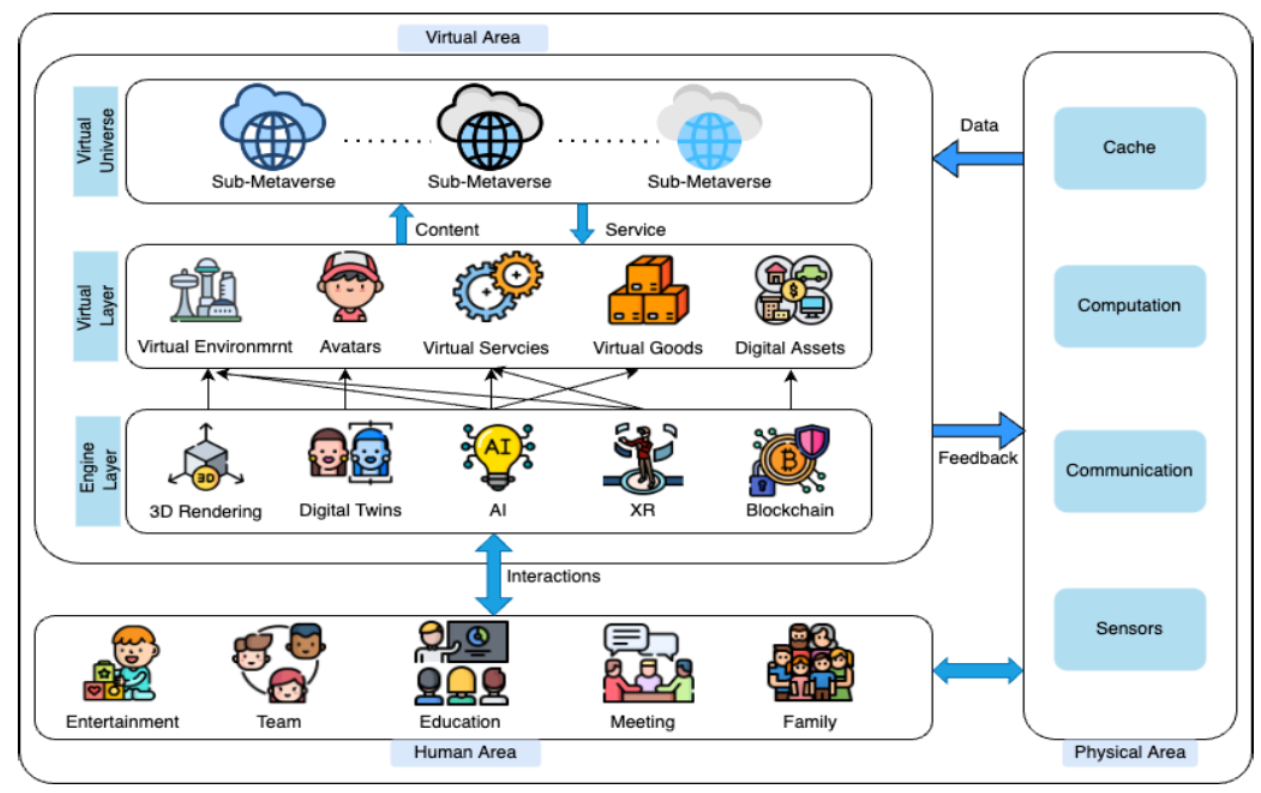
\includegraphics[width=\textwidth]{images/metaverse/metaverseAbstractArchitecture.png}
    \caption{Architektura Metaverse realizuje interakcje pomiędzy obszarem wirtualnym, obszarem ludzkim i obszarem fizycznym\cite{aSurveyofMobileEdgeComputingForMetaverse}}
    \label{abstractMetaverseArchitectureHumanVirtualPhisical}
\end{figure}

Kluczowe cechy metaverse:

\begin{itemize}
    \item Trwałość oznacza, istnienie niezależnie od fizycznej obecności użytkownika\cite{metaverseAFullDive}.
    \item Nieskończoność obsługiwanie niezliczonej liczby użytkowników i światów VR\cite{metaverseAFullDive}.
    \item Samowystarczalność oznacza, że użytkownicy mogą zarabiać w Metaverse i płacić za swoją użyteczność\cite{metaverseAFullDive}.
    \item Interoperacyjność pomaga użytkownikom przenosić ich wirtualne przedmioty, w tym awatary, z jednego projektu Metaverse do drugiego\cite{metaverseAFullDive}.
    \item Czas rzeczywisty pozwala użytkownikom cieszyć się doświadczeniami na żywo\cite{metaverseAFullDive}.
\end{itemize}


Metaverse ma być wciągającym wirtualnym światem, który płynnie łączy sferę fizyczną i cyfrową, umożliwiając użytkownikom interakcję, współpracę i angażowanie się w szereg działań we wspólnym wirtualnym środowisku. U podstaw tej rewolucyjnej koncepcji leży solidna infrastruktura, która służy jako szkielet, ułatwiając płynną łączność i interoperacyjność. Infrastruktura metaverse to ewoluująca, złożona sieć wzajemnie połączonych technologii, protokołów i ram, które współpracują ze sobą w celu stworzenia jednolitego i spójnego wirtualnego wszechświata\cite{metaverseInfrastructureIEEE}.

Infrastruktura ta obejmuje szeroką gamę komponentów, w tym szybkie sieci, potężne zasoby obliczeniowe, zaawansowane urządzenia sprzętowe i najnowocześniejsze platformy oprogramowania. Wykorzystuje ona najnowsze osiągnięcia w takich dziedzinach jak rzeczywistość wirtualna, rzeczywistość rozszerzona, blockchain i zdecentralizowane przetwarzanie danych, aby zapewnić wciągające i bezpieczne doświadczenie metawersji użytkownikom na całym świecie\cite{metaverseInfrastructureIEEE}.

\subsubsection{Architektura sieci w metawersji}

Architektura sieci w metaverse została zaprojektowana tak, aby wspierać płynne interakcje i komunikację w czasie rzeczywistym, umożliwiając użytkownikom angażowanie się w różne działania bez doświadczania opóźnień lub rozłączeń. Wykorzystuje ona zaawansowane protokoły i technologie sieciowe, które priorytetowo traktują niskie opóźnienia, wysoką przepustowość i wydajny transfer danych\cite{metaverseInfrastructureIEEE}.

Zdecentralizowane sieci odgrywają kluczową rolę w zwiększaniu łączności metaverse. Wykorzystując technologię blockchain i sieci peer-to-peer, infrastruktura metaverse ma na celu zmniejszenie zapotrzebowania na centralizacje zarządców lub pośredników. Takie podejście może zapewnić odporność, przejrzystość i demokratyczne zarządzanie, umożliwiając użytkownikom udział w rozwoju metawersji i procesach decyzyjnych\cite{metaverseInfrastructureIEEE}.

Przesyłanie danych i zarządzanie nimi w ramach infrastruktury metaverse jest ułatwione dzięki połączeniu tradycyjnych technologii sieciowych i nowych systemów rozproszonych. Szybkie sieci światłowodowe i łączność bezprzewodowa 5G/6G zapewniają przepustowość niezbędną do przesyłania bogatych treści multimedialnych i strumieni danych w czasie rzeczywistym. Jednocześnie zdecentralizowane rozwiązania pamięci masowej, takie jak rozproszone systemy plików i InterPlanetary File System \akronim{IPFS}, zapewniają bezpieczne i redundantne przechowywanie danych, umożliwiając efektywny dostęp do zasobów cyfrowych i ich wyszukiwania\cite{metaverseInfrastructureIEEE}.

Technologie przetwarzania na krawędzi (\english{Edge Computing}) mogą znacząco przyczynić się do zwiększenia wydajności infrastruktury metaverse. Przybliżając zasoby obliczeniowe do urządzeń brzegowych (takich jak zestawy słuchawkowe VR i okulary AR), przetwarzanie brzegowe zmniejsza opóźnienia i poprawia szybkość reakcji, zwiększając ogólne wrażenia użytkownika. Podejście to odciąża również scentralizowane serwery od zadań przetwarzania, rozkładając obciążenie obliczeniowe na całą sieć i zapewniając skalowalność w miarę wzrostu rozmiaru i złożoności metaverse\cite{metaverseInfrastructureIEEE}.

Technologie blockchain mogą odgrywać kluczową rolę w zwiększaniu bezpieczeństwa sieci w metawersji. Wykorzystując zdecentralizowane mechanizmy konsensusu i protokoły kryptograficzne, blockchain zapewnia integralność i niezmienność danych, chroniąc przed manipulacją i nieautoryzowanym dostępem. Dodatkowo, inteligentne kontrakty ułatwiają bezpieczne i przejrzyste interakcje, automatyzując złożone procesy i umożliwiając transakcje bez zaufania w ramach architektury metaverse i modelowania 3D\cite{metaverseInfrastructureIEEE}.

\subsubsection{Wymagania sprzętowe dla metawersji}

Aby uzyskać dostęp i w pełni doświadczyć metawersji, użytkownicy będą potrzebować specjalistycznego sprzętu, który może obsługiwać wciągające środowiska wirtualne i płynne interakcje. Podstawą tych wymagań sprzętowych są urządzenia komputerowe, takie jak komputery stacjonarne, konsole do gier lub wyspecjalizowane stacje robocze do rozwoju metaverse. Urządzenia te muszą posiadać wystarczającą moc obliczeniową, możliwości graficzne i zasoby pamięci, aby renderować szczegółowe środowiska 3D i obsługiwać złożone symulacje technologii metaverse\cite{metaverseInfrastructureIEEE}.

Infrastruktura metaverse w dużym stopniu wykorzystuje urządzenia rzeczywistości rozszerzonej i wirtualnej, aby zapewnić użytkownikom wciągające wrażenia. Zestawy VR, takie jak Oculus Rift, HTC Vive i PlayStation VR, przenoszą użytkowników do w pełni zrealizowanych wirtualnych światów, umożliwiając im interakcję z cyfrowymi obiektami i awatarami tak, jakby były prawdziwe. Urządzenia AR, takie jak Microsoft HoloLens i Magic Leap One, płynnie łączą elementy cyfrowe ze światem fizycznym, umożliwiając użytkownikom rozszerzenie otoczenia o wirtualne nakładki i interaktywne interfejsy\cite{metaverseInfrastructureIEEE}.

Zaawansowane jednostki przetwarzające, w tym wysokowydajne procesory graficzne \akronim{GPU} (\english{Graphics Processing Unit}) i wyspecjalizowane akceleratory, odgrywają kluczową rolę w zwiększaniu doznań płynących z metaverse. Komponenty te są odpowiedzialne za renderowanie złożonych środowisk 3D, symulację fizyki i przetwarzanie ogromnych ilości danych w czasie rzeczywistym. Dodatkowo, integracja sztucznej inteligencji i technologii uczenia maszynowego w infrastrukturze metaverse wymaga potężnych zasobów obliczeniowych, aby umożliwić inteligentne interakcje, przetwarzanie języka naturalnego i realistyczne awatary\cite{metaverseInfrastructureIEEE}.

Wraz z ciągłym rozwojem technologii, infrastruktura metaverse dostosowuje się do nowych technologii, które mogą jeszcze bardziej poprawić wrażenia użytkownika. Przykładowo, rozwój interfejsów mózg-komputer \akronim{BCI} (\english{Brain-Computer Interface}) i haptycznych urządzeń sprzężenia zwrotnego może zrewolucjonizować sposób interakcji użytkowników ze środowiskami wirtualnymi, umożliwiając bardziej intuicyjne i wciągające doświadczenia. Co więcej, postępy w dziedzinie obliczeń kwantowych i przetwarzania fotonicznego mogą potencjalnie zrewolucjonizować metawersję, zapewniając bezprecedensową moc obliczeniową a co za tym idzie możliwości przetwarzania danych\cite{metaverseInfrastructureIEEE}.

\subsubsection{Transakcje w metawersji}

Wirtualne waluty i technologia blockchain znajdują się w czołówce, jeśli chodzi o ułatwianie transakcji w metaverse. Te cyfrowe aktywa, często określane jako kryptowaluty lub tokeny, mogą służyć jako podstawowy środek wymiany towarów, usług i wirtualnych aktywów w wirtualnym środowisku metaverse. Wykorzystując zdecentralizowany i bezpieczny charakter technologii blockchain, te wirtualne waluty umożliwiają płynne, przejrzyste i pozbawione zaufania transakcje, eliminując potrzebę pośredników i zmniejszając koszty transakcji\cite{metaverseInfrastructureIEEE}.

Inteligentne kontrakty, które są samowykonalnymi umowami zakodowanymi w sieciach blockchain, mogą odgrywać kluczową rolę w automatyzacji i zabezpieczaniu transakcji w metaverse. Kontrakty te definiują zasady i warunki różnych umów, takich jak transfery aktywów, umowy o świadczenie usług i rozliczenia finansowe. Po wdrożeniu, inteligentne kontrakty wykonują się automatycznie, gdy spełnione są wcześniej określone warunki, zapewniając przejrzystość, wydajność i niezmienne prowadzenie dokumentacji dla wszystkich transakcji w ramach immersyjnego doświadczenia metaverse\cite{metaverseInfrastructureIEEE}.

Aktywami cyfrowymi i własnością intelektualną można zarządzać poprzez połączenie technologii blockchain i zdecentralizowanych rozwiązań w zakresie przechowywania. Tokeny niewymienialne \akronim{NFT} (\english{Non-Fungible Token}) mogą być wykorzystywane do reprezentowania unikalnych zasobów cyfrowych, takich jak wirtualne nieruchomości, dzieła sztuki, przedmioty kolekcjonerskie i przedmioty w grze. Tokeny te są przechowywane w sieciach blockchain, zapewniając łatwą weryfikację własności i pochodzenia. Ponadto zdecentralizowane systemy przechowywania plików, takie jak IPFS, umożliwiają bezpieczne i redundantne przechowywanie treści cyfrowych, zapewniając długowieczność i dostępność wirtualnych zasobów\cite{metaverseInfrastructureIEEE}.

Infrastruktura metaverse może ułatwiać wirtualne rynki i interakcje gospodarcze poprzez integrację zdecentralizowanych aplikacji \akronim{dApps} (\english{Decentralized application}) i zdecentralizowanych protokołów finansowych \akronim{DeFi} (\english{decentralized finance}). Platformy te umożliwiają użytkownikom kupowanie, sprzedawanie, handlowanie i inwestowanie w szeroką gamę wirtualnych aktywów, towarów i usług. Inteligentne kontrakty automatyzują i zarządzają tymi transakcjami, zapewniając uczciwość, przejrzystość i przestrzeganie wcześniej określonych zasad. Co więcej, zdecentralizowane autonomiczne organizacje \akronim{DAO} (\english{Decentralized autonomous organization}) pozwalają na zbiorowe podejmowanie decyzji i zarządzanie w ramach tych wirtualnych rynków, wspierając poczucie wspólnoty i współwłasności\cite{metaverseInfrastructureIEEE}.

\subsubsection{Ekosystem Metaverse}

\begin{figure}[!htbp]
    \centering
    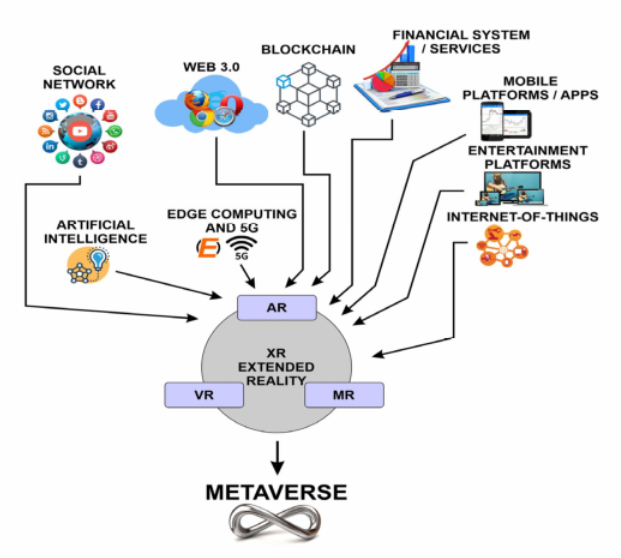
\includegraphics[width=\textwidth]{images/metaverse/metaverseEcosystem.png}
    \caption{Ekosystem Metaverse\cite{metaverseSecurityIssuesChallengesAndViableZTAModel}}
    \label{metaverseEcosystemImage}
\end{figure}

Metaverse umożliwia realizację kilku nowatorskich scenariuszy biznesowych w wielu różnych branżach. Połączenie tych technologii w połączeniu z nowymi rozwiązaniami pomoże zrealizować wizję metawersji w przyszłości. Rysunek \ref{metaverseEcosystemImage} przedstawia nadrzędny ekosystem technologiczny umożliwiający powstanie metawersji. Nie ulega wątpliwości, że technologie AR/VR/MR i XR stanowią podstawę metawersji, umożliwiając użytkownikom dostęp do wirtualnego świata 3D. W swojej najwcześniejszej iteracji metaverse może być zbiorem aplikacji Web 3.0 z XR-Skin zapewniającym ograniczone wrażenia VR. Oczekuje się, że sieci społecznościowe będą jednymi z pierwszych, które przeniosą się do metaverse, umożliwiając użytkownikom udostępnianie i konsumowanie treści immersyjnych wraz z Web 3.0, umożliwiając firmom oferowanie użytkownikom nowatorskich doświadczeń produktowych. Technologia blockchain zostanie szeroko wdrożona w metaverse, aby umożliwić realizację wizji zdecentralizowanych finansów i gospodarki twórców, które są nowymi tematami, głównie ze względu na bezpieczeństwo i prywatność, które oferują. Aplikacje i platformy mobilne mogą być kolejnymi, które migrują do metaverse, a następnie platformy rozrywkowe. Wreszcie, łączność 5G/6G, oferująca niskie opóźnienia, może być spoiwem, które płynnie połączy wszystkie elementy, podczas gdy Internet Rzeczy będzie łączył wszystkie urządzenia wraz z intensywnym wykorzystaniem sztucznej inteligencji, w tym inteligencji brzegowej, w celu zapewnienia spersonalizowanych doświadczeń\cite{metaverseSecurityIssuesChallengesAndViableZTAModel}. 
Można przewidzieć, że ekosystem metaverse przedstawiony na rysunku \ref{metaverseEcosystemImage} może przyjąć trzy potencjalne ścieżki ewolucji:

\begin{itemize}
    \item Zamknięty Metaverse: Dla niszowych aplikacji i przypadków użycia ograniczonych do użytku przez konkretną społeczność o wyspecjalizowanych potrzebach.
    \item Federacyjny: Zarządzana i obsługiwana przez dużą korporację z ekosystemem współpracujących partnerów, zewnętrznych dostawców i usługodawców dostarczających użytkownikom końcowym ujednolicone doświadczenie;  
    \item Otwarty Metaverse: Metawersja niesfederowana, nie kontrolowana przez żaden pojedynczy podmiot. O otwartej architekturze i społeczności deweloperów tworzących aplikacje/usługi dla użytkowników końcowych.
\end{itemize}



Prawdopodobnym jest, że ekosystem metaverse, jak pokazano na rysunku \ref{metaverseEcosystemImage}, może przyjąć trzy formy. Można oczekiwać, że wszystkie trzy modele będą współistnieć w takiej czy innej formie. Meta Facebooka jest doskonałym przykładem metawersji federacyjnej\cite{metaverseSecurityIssuesChallengesAndViableZTAModel}. 

Oczekuje się, że w przyszłości pojawią się inne modele, głównie napędzane przez sojusze biznesowe, fuzje i przejęcia. Jest prawdopodobne, że metaverse napotka kilka przeszkód na drodze do jego szerokiego przyjęcia. Niektóre z wyzwań stojących na drodze do realizacji pełnego potencjału koncepcji metaverse i jej przyjęcia obejmują:

\begin{itemize}
    \item Dostęp: Obecnie tylko przez zestawy okularów wirtualnej rzeczywistości, które nie są aktualnie powszechne
    \item Łatwość użytkowania: Użytkownicy uważają, że obecna wersja zestawów okularów wirtualnej rzeczywistości jest nieporęczna i trudna do noszenia przez długi czas
    \item Brak rozwiniętego ekosystemu: Niewiele aplikacji dostępnych na obecnych platformach VR
    \item Bezpieczeństwo i prywatność: Środowiska XR cierpią z powodu luk w zabezpieczeniach podstawowych technologii, w tym kwestii dotyczących prywatności użytkowników w wirtualnych światach. 
\end{itemize}

Podczas gdy oczekuje się, że postęp technologiczny rozwiąże kwestie dostępu i łatwości użytkowania w najbliższej przyszłości, kwestie bezpieczeństwa i prywatności muszą być budowane od podstaw podczas projektowania ekosystemu metaverse\cite{metaverseSecurityIssuesChallengesAndViableZTAModel}. 


\subsubsection{Podsumowanie}

Metawersja stanowi rewolucyjny skok w sposobie, w jaki ludzie postrzegają środowiska cyfrowe i wchodzą z nimi w interakcję, zacierając granice między sferą fizyczną i wirtualną. U podstaw tej koncepcji leży wiele koncepcji solidnej i zaawansowanej infrastruktury, która posłuży jako podstawa płynnej łączności, wciągających doświadczeń i nieograniczonych możliwości. 

W miarę jak metawersja będzie ewoluować i zyskiwać popularność, jej infrastruktura będzie odgrywać kluczową rolę w kształtowaniu przyszłości cyfrowych interakcji, handlu i kontaktów społecznych. Wykorzystując najnowocześniejsze technologie, takie jak blockchain, rzeczywistość wirtualna, rzeczywistość rozszerzona i zdecentralizowane przetwarzanie, infrastruktura metaverse umożliwia bezpieczne, przejrzyste i interoperacyjne przestrzenie wirtualne.

Pomyślne wdrożenie i rozwój metawersji będzie jednak również wymagać sprostania krytycznym wyzwaniom związanym z zarządzaniem, regulacjami, bezpieczeństwem i prywatnością. Współpraca między zainteresowanymi stronami, w tym deweloperami, decydentami i szerszą społecznością, jest niezbędna do ustanowienia skutecznych ram, które sprzyjają innowacjom, jednocześnie chroniąc użytkowników i utrzymując standardy etyczne.
\chapter{Metaverse --- przegląd literatury}

Niniejszy rozdział przedstawia obecne implementacje Metaverse, podkreślając technologiczne podstawy i wyzwania stojące przed realizacją tego rozwijającego się wirtualnego środowiska. Zaprezentowane informacje oparte są na analizie wybranych artykułów naukowych.

\section{A Survey of Mobile Edge Computing for the
Metaverse: Architectures, Applications, and
Challenges}

Artykuł "A Survey of Mobile Edge Computing for the Metaverse: Architectures, Applications, and Challenges" autorstwa Yitong Wang i Jun Zhao z Nanyang Technological University Singapore bada przede wszystkim możliwość wykorzystania Mobile Edge Computing \akronim{MEC} w środowisku Metaverse, podkreślając aspekty techniczne i infrastrukturę wymaganą do obsługi tak złożonego systemu.

\akronim{MEC} jest definiowany jako rozproszony paradygmat obliczeniowy, który umieszcza zasoby obliczeniowe i pamięć masową na urządzeniach końcowych, w celu realizacji przetwarzania na tych urządzeniach. Zmniejsza to opóźnienia i poprawia wydajność aplikacji poprzez przeniesienie intensywnych zadań na pobliskie serwery brzegowe.

\subsection{Infrastruktura sieciowa}

Wdrożenie sieci \akronim{5G} ma kluczowe znaczenie dla Metaverse ze względu na wysoką szybkość transmisji danych, niskie opóźnienia i wysoką gęstość połączeń. Integracja \akronim{MEC} z sieciami \akronim{5G} zapewnia, że dane generowane przez urządzenia, takie jak zestawy VR, mogą być przetwarzane szybko i wydajnie.

Serwery zlokalizowane na brzegu sieci, wykonują zadania obliczeniowe odciążające urządzenia końcowe, zmniejszając w ten sposób obciążenie sieci rdzeniowych i zapewniając przetwarzanie w czasie rzeczywistym.

\subsection{Paradygmaty obliczeniowe}

Podczas gdy tradycyjne przetwarzanie w chmurze aktualnie odgrywa kluczową rolę w systemach rozproszonych, poleganie wyłącznie na serwerach w chmurze może powodować duże opóźnienia i przeciążenia sieci. Dlatego konieczne jest podejście hybrydowe obejmujące przetwarzanie brzegowe i przetwarzanie we mgle (\english{fog computing}).

Przetwarzanie we mgle działa jako warstwa pośrednia między chmurą a urządzeniami brzegowymi, obsługując zadania, które wymagają mniejszych opóźnień niż może zaoferować chmura, ale są zbyt intensywne dla samych urządzeń brzegowych.

\subsection{Transmisja i przetwarzanie danych}

Przetwarzając dane bliżej źródła ich generowania (np. na serwerach brzegowych), MEC znacznie zmniejsza opóźnienia w porównaniu z tradycyjnymi rozwiązaniami opartymi na chmurze. Ma to kluczowe znaczenie dla immersyjnych doświadczeń w czasie rzeczywistym wymaganych w Metaverse.

\akronim{MEC} pomaga w zarządzaniu wykładniczym wzrostem ruchu danych poprzez przetwarzanie i filtrowanie danych na krawędzi przed przesłaniem ich do chmury, optymalizując w ten sposób wykorzystanie przepustowości

\subsection{Modele architektury}

Architektura Metaverse oparta na \akronim{MEC}, zaprezentowana na rys.\ref{mecBaseArch} obejmuje dynamiczne węzły brzegowe do obsługi interakcji użytkownika i przetwarzania danych, minimalizując w ten sposób opóźnienia i poprawiając doświadczenia świadczonych usług przez użytkownika.

\begin{figure}[htbp!]
    \centering
    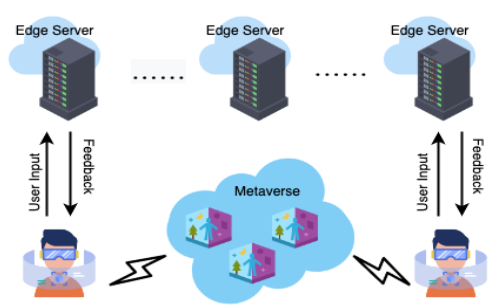
\includegraphics[width=0.85\textwidth]{images/existingArchitectres/mecBaseArch.png}
    \caption{Architektura Metaverse wykorzystująca Mobile Edge Computing}
    \label{mecBaseArch}
\end{figure}

\newpage
Architektura oparta na przetwarzaniu we mgle proponuje wielopoziomowe podejście, w którym różne zadania obliczeniowe są dystrybuowane w warstwach mgły, krawędzi i chmury w celu optymalizacji wydajności i zmniejszenia wąskich gardeł obliczeniowych.

Artykuł podkreśla znaczenie \akronim{MEC} w infrastrukturze Metaverse poprzez rozwiązywanie krytycznych kwestii, takich jak opóźnienia, wydajność przepustowości i zarządzanie zasobami obliczeniowymi. Przybliżając moc obliczeniową do użytkowników końcowych i wykorzystując zaawansowaną infrastrukturę sieciową, taką jak \akronim{5G}, paradygmat \akronim{MEC} jest niezbędny do implementacji świata Metaverse.

\section{Dynamic Resource Allocation for Metaverse Applications with Deep Reinforcement Learning}

Artykuł "Dynamic Resource Allocation for Metaverse Applications with Deep Reinforcement Learning" autorstwa Nam H. Chu,
Eryk Dutkiewicz, Diep N. Nguyen, Dinh Thai Hoang, Khoa T. Phan, Dusit Niyato i Tao Shu koncentruje się na infrastrukturze i aspektach technicznych wymaganych do efektywnego zarządzania ogromnym zapotrzebowaniem na zasoby aplikacji Metaverse.

\subsection{Wyzwania związane z zarządzaniem zasobami}

Autorzy w artykule wskazują następujące wyzwania związane z zarządzaniem zasobami w środowisku Metaverse:

\begin{itemize}
    \item Aplikacje Metaverse wymagają dużych zasobów obliczeniowych, pamięci masowej i sieci, które przekraczają możliwości istniejących systemów.
    \item Dynamiczny i niepewny charakter żądań użytkowników i cykli życia aplikacji wymaga zaawansowanych strategii zarządzania zasobami.
\end{itemize}

\subsection{Proponowane rozwiązania}

Autorzy proponują następujące rozwiązania:
\begin{itemize}
    \item MetaInstancje i MetaSlices --- Aplikacje są podzielone na MetaInstancje, w których funkcje mogą być współdzielone między aplikacjami w celu zwiększenia efektywności wykorzystania zasobów.
    \item Architektura wielowarstwowa --- Framework wykorzystuje wielowarstwową architekturę chmury obliczeniowej do efektywnej dystrybucji zasobów z chmury do brzegu sieci, zmniejszając opóźnienia i przeciążenia.
\end{itemize}

\subsection{Wielowarstwowa architektura obliczeniowa}

Warstwowa dystrybucja zasobów zaprezentowana na rys.\ref{metaslicingMultiTierArch} zapewnia, że zasoby są dystrybuowane na wielu poziomach, od użytkowników końcowych po serwery w chmurze, aby zrównoważyć obciążenie i zoptymalizować wydajność.

\begin{figure}[!htbp]
    \centering
    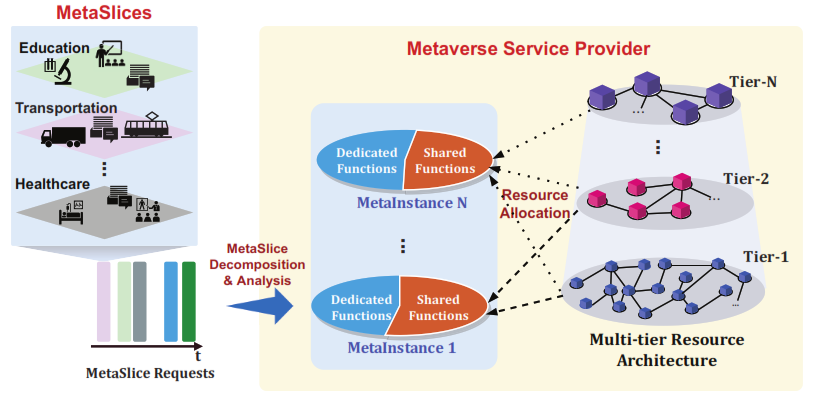
\includegraphics[width=\textwidth]{images/existingArchitectres/dynamicResourcemetaslicingMultiTierArch.png}
    \caption{Warstwowa dystrybucja zasobów}
    \label{metaslicingMultiTierArch}
\end{figure}

Dekompozycja aplikacji powoduje że aplikacje są dzielone na mniejsze funkcje, z których każda jest wykonywana na różnych poziomach w oparciu o ich wymagania dotyczące zasobów i dostępne możliwości.

Artykuł przedstawia zaawansowany framework do dynamicznego zarządzania i alokacji zasobów w Metaverse przy użyciu kombinacji wielowarstwowego przetwarzania w chmurze i zaawansowanych technik głębokiego uczenia ze wzmocnieniem. Dzięki dekompozycji aplikacji na MetaSlices i MetaInstances oraz zastosowaniu procesu decyzyjnego semi-Markova, framework skutecznie radzi sobie z ogromnym i dynamicznym zapotrzebowaniem na zasoby aplikacji Metaverse.

\section{Unlocking Metaverse-as-a-Service}

Artykuł "Unlocking Metaverse-as-a-Service" autorstwa Vesal Ahsani, Ali Rahimi, 
Mehdi Letafati, Babak Hossein Khalaj, omawia niezbędną infrastrukturę techniczną i wyzwania związane z wdrażaniem platform Metaverse-as-a-Service \akronim{MaaS}.

\subsection{Główne filary MaaS}

Autorzy wskazują trzy główne filary:
\begin{itemize}
    \item Prywatność i bezpieczeństwo --- Zapewnienie bezpiecznych i prywatnych interakcji w Metaverse jest najważniejsze. Artykuł kładzie nacisk na mechanizmy prywatyzacji wrażliwych atrybutów danych i zabezpieczania rozproszonych algorytmów uczenia maszynowego.
    \item Przetwarzanie brzegowe --- wzmacnia Metaverse poprzez zmniejszenie opóźnień i przeciążenia sieci. Obejmuje przetwarzanie i przechowywanie danych blisko użytkowników końcowych, zwiększając wydajność i skalowalność aplikacji Metaverse
    \item Technologia Blockchain --- Blockchain zapewnia przejrzystość, integralność danych i bezpieczne transakcje w ramach Metaverse. Obsługuje zdecentralizowane aplikacje i inteligentne kontrakty, niezbędne dla ekonomicznej i operacyjnej integralności Metaverse.
\end{itemize}

\subsection{Przetwarzanie brzegowe w Maas}

Struktura \akronim{MaaS} opiera się w dużej mierze na przetwarzaniu brzegowym, w którym przetwarzanie i przechowywanie danych odbywa się blisko użytkowników, zmniejszając opóźnienia i poprawiając wrażenia użytkownika. Serwery brzegowe mają kluczowe znaczenie dla obsługi lokalnego przetwarzania danych, pamięci masowej i funkcji sieciowych. Odciążają intensywne zadania z centralnych serwerów w chmurze, optymalizując ruch sieciowy i zwiększając możliwości przetwarzania danych w czasie rzeczywistym.

\subsection{Infrastruktura sieciowa}

Sieci 5G/6G --- Szybkie sieci bezprzewodowe o niskich opóźnieniach są niezbędne do obsługi wymagań Metaverse w czasie rzeczywistym. Sieci te ułatwiają płynny transfer danych między urządzeniami brzegowymi a serwerami. 

Bramy internetowe --- Łączą one systemy brzegowe z szerszą infrastrukturą sieciową i chmurową, zapewniając wydajny przepływ danych.

\subsection{Zarządzanie danymi i bezpieczeństwo}

Kontrola danych --- Przetwarzanie brzegowe zwiększa kontrolę nad danymi, utrzymując je blisko źródła, zapewniając lepsze zarządzanie prywatnością i bezpieczeństwem. Ma to kluczowe znaczenie dla obsługi danych wrażliwych, takich jak dane biometryczne i informacje zdrowotne.
Bezpieczna wymiana danych: Technologia Blockchain zapewnia, że dane udostępniane w ramach Metaverse są bezpieczne i niezmienne. Technologia ta wspiera bezpieczne transakcje i interakcje między użytkownikami i aplikacjami.

\subsection{Optymalizacja wydajności}

Przetwarzając dane na brzegu sieci, platforma znacząco redukuje opóźnienia, co ma kluczowe znaczenie dla aplikacji działających w czasie rzeczywistym, takich jak AR/VR i interaktywne gry.
Przetwarzanie brzegowe optymalizuje przepustowość sieci poprzez lokalne przetwarzanie danych, zmniejszając potrzebę przesyłania dużych ilości danych do centralnych serwerów.

Artykuł przedstawia infrastrukturę techniczną wymaganą do obsługi platform Metaverse-as-a-Service, koncentrując się na prywatności i bezpieczeństwie, przetwarzaniu brzegowym i technologii blockchain. Przetwarzanie brzegowe odgrywa kluczową rolę w zmniejszaniu opóźnień i optymalizacji wydajności sieci, podczas gdy blockchain zapewnia integralność danych i bezpieczne transakcje. Integracja tych technologii tworzy solidne, skalowalne i bezpieczne ramy dla Metaverse, zdolne do obsługi rozległych i dynamicznych wymagań dotyczących zasobów w immersyjnych środowiskach wirtualnych.


\section{Porównanie i podsumowanie}

Wszystkie trzy artykuły podkreślają kluczową rolę zaawansowanych technologii i infrastruktury we wdrażaniu środowiska Metaverse. W szczególności omówione prace analizują komponenty niezbędne dla działania tego środowiska i wyzwania stawiane przed jego twórcami. Poddane analizie prace skupiają się w szczególności na następujących aspektach: 
\begin{itemize}
    \item Koncentracja na zaawansowanych technologiach:
    \begin{itemize}
        \item Wszystkie artykuły podkreślają znaczenie zaawansowanych technologii, takich jak przetwarzanie brzegowe i sieci \akronim{5G/6G} we wdrażaniu aplikacji Metaverse.
        \item Podkreślają potrzebę skalowalnego, wydajnego zarządzania zasobami w celu obsługi wysokich wymagań aplikacji Metaverse.
    \end{itemize}
    \item Wymagania dotyczące infrastruktury:
    \begin{itemize}
        \item Artykuły omawiają krytyczne komponenty infrastruktury niezbędne dla Metaverse, w tym serwery brzegowe, przetwarzanie w chmurze i architekturę sieci.
        \item Wszystkie artykuły podkreślają rolę przetwarzania brzegowego w zmniejszaniu opóźnień i poprawie wydajności poprzez przetwarzanie danych bliżej źródła.
    \end{itemize}
    \item Wyzwania związane z wdrażaniem Metaverse:
    \begin{itemize}
        \item Wszystkie artykuły dostrzegają wyzwania związane z wdrażaniem aplikacji Metaverse, takie jak opóźnienia, wydajność przepustowości i potrzeba przetwarzania w czasie rzeczywistym.
        \item Uznają one trudności w zarządzaniu ogromnymi danymi i wymaganiami obliczeniowymi aplikacji Metaverse.
    \end{itemize}
\end{itemize}

Chociaż artykuły mają wspólną płaszczyznę, koncentrując się na technologicznych podstawach Metaverse, różnią się one w swoich konkretnych podejściach, ramach i obszarach nacisku. Kluczowe różnice między tymi badaniami to:
\begin{itemize}
    \item Konkretne obszary tematyczne:
    \begin{itemize}
        \item "A Survey of Mobile Edge Computing for the Metaverse: Architectures, Applications, and Challenges": Ten artykuł koncentruje się na integracji Mobile Edge Computing z Metaverse, szczegółowo opisując architektury, aplikacje i wyzwania związane z tą integracją.
        \item "Dynamic Resource Allocation for Metaverse Applications with Deep Reinforcement Learning": Ten artykuł koncentruje się na dynamicznej alokacji zasobów przy użyciu technik głębokiego uczenia się ze wzmocnieniem, zapewniając szczegółowe frameworki i inteligentny algorytm optymalizacji zarządzania zasobami w Metaverse.
        \item "Unlocking Metaverse-as-a-Service": Ten artykuł podkreśla koncepcję Metaverse-as-a-Service, koncentrując się na prywatności i bezpieczeństwie, przetwarzaniu brzegowym i technologii blockchain jako głównych filarach wspierających infrastrukturę MaaS.
    \end{itemize}
    \item Podejście do zarządzania zasobami:
    \begin{itemize}
        \item  Pierwszy artykuł podkreśla rolę MEC w ulepszaniu aplikacji Metaverse poprzez zmniejszenie opóźnień i poprawę wydajności przetwarzania danych poprzez przetwarzanie brzegowe.
        Drugi artykuł koncentruje się na wykorzystaniu głębokiego uczenia ze wzmocnieniem do dynamicznego przydzielania zasobów, prezentując podejście algorytmiczne do zarządzania wysokim i zmiennym zapotrzebowaniem na zasoby aplikacji Metaverse.
        W artykule MaaS omówiono, w jaki sposób MaaS może być wykorzystywany do świadczenia skalowalnych usług na żądanie, podkreślając integrację przetwarzania brzegowego i łańcucha bloków w celu zapewnienia bezpiecznych, wydajnych i skalowalnych usług Metaverse.
    \end{itemize}
    \item Szczegóły infrastruktury sieciowej:
    \begin{itemize}
        \item Artykuł MEC zagłębia się w specyfikę architektur sieciowych niezbędnych do integracji MEC z sieciami \akronim{5G}, podkreślając, w jaki sposób serwery brzegowe mogą odciążać zadania z urządzeń końcowych.
        \item Artykuł dotyczący dynamicznej alokacji zasobów proponuje wielowarstwową architekturę chmury obliczeniowej w celu efektywnej dystrybucji zasobów, eliminacji wąskich gardeł obliczeniowych i optymalizacji wydajności poprzez podejście warstwowe.
        \item Artykuł MaaS omawia, w jaki sposób technologia blockchain może zostać zintegrowana z infrastrukturą Metaverse w celu zwiększenia bezpieczeństwa, przejrzystości i integralności danych, uzupełniając podejście Edge Computing w celu zmniejszenia opóźnień i poprawy świadczenia usług.
    \end{itemize}
    \item Transmisja i przetwarzanie danych:
    \begin{itemize}
        \item W artykule poświęconym MEC omówiono korzyści płynące z przetwarzania danych na brzegu sieci w celu zmniejszenia opóźnień i bardziej efektywnego zarządzania ruchem danych.
        \item Drugi artykuł kładzie nacisk na zarządzanie zasobami w czasie rzeczywistym przy użyciu zaawansowanych algorytmów w celu zapewnienia optymalnej wydajności i jakości usług w Metaverse.
        \item Artykuł MaaS podkreśla znaczenie bezpiecznej obsługi danych i prywatności, wykorzystując blockchain w celu zapewnienia integralności danych i przetwarzania brzegowego w celu wydajnego przetwarzania w czasie rzeczywistym.
    \end{itemize}
\end{itemize}

Wszystkie trzy artykuły wnoszą cenny wkład w infrastrukturę techniczną i strategie zarządzania zasobami niezbędne do wdrożenia Metaverse. Są one podobne pod względem skupienia się na zaawansowanych technologiach i wyzwaniach, ale różnią się konkretnymi podejściami i szczegółowymi frameworkami. Artykuł koncentrujący się na MEC zapewnia szerszy przegląd architektur sieciowych i przetwarzania brzegowego, artykuł o alokacji zasobów oferuje głębokie zanurzenie w algorytmicznych rozwiązaniach do zarządzania zasobami w czasie rzeczywistym, a artykuł MaaS kładzie nacisk na integrację przetwarzania brzegowego i blockchain w celu stworzenia skalowalnej i bezpiecznej platformy Metaverse-as-a-Service.
\chapter{Implementacja}
% Temporarily change the margins for this page
\newgeometry{
  left=0.5in,
  right=0.5in,
  top=1.5in,
  bottom=1in,
}
\section{Elementy tworzonego systemu}
\begin{figure}[!htbp]
    \centering
    \includesvg[width=\textwidth]{schemas/master-Dev.drawio.svg}
    \caption{Schemat tworzonego systemu}
    \label{fig:enter-label}
\end{figure}

% Restore the original margins
\restoregeometry
\newpage

\begin{figure}[h!]
    \centering
    \begin{msc}[
        title position=center,
        msc keyword=,
        draw frame=none,
        instance distance=2.5cm,
        left environment distance=0.5cm,
        right environment distance=0.5cm,
        label distance=0.3cm,
        title distance=0.5cm
        ]{Protocol Worker Resource Reservation}
            \declinst{user}{}{User}
            \declinst{protocolWorker}{}{Protocol Worker}
            \declinst{serviceDiscovery}{}{Service Discovery}
            \declinst{producer}{}{Producer}
            
            \footnotesize
            \nextlevel
            \mess{Request Resource Reservation}{user}{protocolWorker}
            \nextlevel
            \nextlevel
            \mess{Query All Registered Producers}{protocolWorker}{serviceDiscovery}
            \nextlevel
            \nextlevel
            \nextlevel
            \mess{List of Producers}{serviceDiscovery}{protocolWorker}
            \nextlevel
            \nextlevel
            \nextlevel
            \inlinestart{loop1}{loop for each Producer}{protocolWorker}{producer}
            \nextlevel
            \nextlevel
            \nextlevel
            \nextlevel
            \mess{Check Resource Availability}{protocolWorker}{producer}
            \nextlevel
            \nextlevel
            \nextlevel
            \mess{Resource Availability}{producer}{protocolWorker}
            \nextlevel
            \nextlevel
            \inlineend{loop1}
            \nextlevel
            \nextlevel
            \mess{\parbox{3cm}{Processing producers for products}}{protocolWorker}{protocolWorker}
            \nextlevel
            \nextlevel
            \nextlevel
            \nextlevel
            \nextlevel
            \mess{Return Resource Availability}{protocolWorker}{user}
        \end{msc}
    \caption{ Schemat wymiany wiadomości podczas przetwarzania żądania użytkownika}
    \label{fig:enter-label}
\end{figure}

\subsection{Producent}
\subsection{Rejestr usług}
\subsection{Węzeł protokołu}
\subsubsection{Podsystem monitoringu producentów}
\subsubsection{Podsystem propozycji zasobów}

\section{Uruchomienie środowiska}
\chapter{Wybrane narzędzia i technologie}


W pracy magisterskiej podczas opracowywania i wdrażania systemu wykorzystano rozmaite narzędzia i technologie. Każde narzędzie odgrywa kluczową rolę w zapewnieniu wydajności, skalowalności i łatwości utrzymania systemu.

\section{Java}

\begin{figure}[!htbp]
    \centering
    
\includegraphics[width=0.1\textwidth]{images/javaLogo.png}
    \caption{Oficjalne logo języka Java}
    \label{fig:enter-label}
\end{figure}

Java jest to szeroko stosowany obiektowy język programowania i platforma oprogramowania, która działa na miliardach urządzeń. Zasady oraz składnia języka zostały oparte na językach \acronym{C} i \acronym{C++}\cite{javaIBM}\cite{cstandard}\cite{cppstandard}. Java powstała aby udoskonalić i naprawić wiele błędnych konceptów wprowadzonych przez te języki. Jedną z głównych zalet tworzenia oprogramowania w Javie jest jej przenoszalność. Po napisaniu kodu programu na jednym urządzeniu można go łatwo przenieść na inne urządzenie o innej architekturze. Język ten został wynaleziony w 1995 roku przez Jamesa Goslinga z Sun Microsystems (później przejętego przez Oracle), główną ideą jego wynalezienia była możliwość, \definicja{"napisania raz, uruchomienia w dowolnym miejscu"}  (\english{write once, run anywhere}). Nowe i ulepszone narzędzia do tworzenia oprogramowania pojawiają się na rynku w niezwykłym tempie, wypierając dotychczasowe produkty, które kiedyś uważano za niezbędne. W świetle tej ciągłej rotacji, trwałość i ciągła popularność języka Java jest imponująca, prawie trzy dekady po jej stworzeniu, Java jest nadal jednym z najbardziej popularnych języków do tworzenia oprogramowania użytkowego\cite{javaIBM}\cite{javaDEV}.

Wszystkie języki programowania służą do komunikacji z maszynami. Sprzęt maszynowy reaguje tylko na komunikację elektroniczną. Języki programowania wysokiego poziomu, takie jak Java, działają jako pomost między językiem ludzkim a językiem sprzętu. Aby korzystać z języka Java, programista powinien mieć świadomość istnienia dwóch poziomów abstrakcji pisanych programów: 

\begin{itemize}
    \item Język Java i \definicja{interfejsy \acronym{API} }(\english{application programming interface})
    \item Wirtualna maszyna Java \acronym{JVM} (\english{\termdef{Java Virtual Machine}})
\end{itemize}

Java definiuje składnię i semantykę języka. Obejmuje to podstawowe słownictwo i reguły używane do pisania algorytmów. 
Interfejsy API są ważnymi komponentami oprogramowania dołączonymi do platformy Java. Są to wstępnie napisane programy, które można podłączyć i odtworzyć istniejące funkcjonalności we własnym kodzie. Na przykład można użyć interfejsów API Java, aby uzyskać datę i godzinę, wykonać operacje matematyczne lub manipulować tekstem. Każdy kod aplikacji Java napisany przez programistę zazwyczaj łączy nowy i wcześniej istniejący kod z interfejsów API Java, bibliotek i frameworków\cite{frameworkDef}\cite{javaAmazon}\cite{javaDEV}.

Wirtualna maszyna Javy działa jako dodatkowa warstwa abstrakcji między platformą Java a sprzętem maszyny. Kod źródłowy Java może działać tylko na tych maszynach na których zainstalowano JVM. Kiedy po raz pierwszy opracowano języki programowania, dzieliły się one na dwie szerokie kategorie, w zależności od tego, w jaki sposób komunikowały się ze sprzętem: 

\begin{itemize}
    \item \textbf{Kompilowany} --- program jest napisany w składni języka, a następnie kompilator tłumaczy cały kod na kod maszynowy. Skompilowany kod jest następnie uruchamiany na sprzęcie.
    \item \textbf{Interpretowany} --- Dzięki interpreterom każda instrukcja kodu wysokiego poziomu jest na bieżąco interpretowana na kod maszynowy. Napisane instrukcje są natychmiast uruchamiane przez sprzęt przed przejściem do następnej instrukcji
\end{itemize}

Język Java był pierwszym językiem, który połączył obie powyższe metody, przy użyciu JVM. Każdy plik programu jest najpierw kompilowany do kodu bajtowego (\english{bytecode}). Kod bajtowy Java może być uruchamiany tylko w maszynie JVM. Następnie JVM interpretuje kod bajtowy, aby uruchomić go na podstawowej platformie sprzętowej. Jeżeli aplikacja działa na komputerze z systemem Windows, maszyna JVM zinterpretuje ją dla systemu Windows. Natomiast jeżeli aplikacja uruchomiona jest na platformie open--source, takiej jak Linux, JVM zinterpretuje ją dla systemu Linux\cite{javaAmazon}\cite{javaDEV}.

\section{Maven}

\begin{figure}[htbp!]
    \centering
    
\includegraphics[width=0.2\textwidth]{images/mavenLogo.png}
    \caption{Logo programu Apache Maven\cite{mavenSite}.}
    \label{fig:enter-label}
\end{figure}

Słowo maven  w języku jidysz oznacza gromadzenie wiedzy. Apache Maven to narzędzie do zarządzania projektami oprogramowania. Opiera się ono na koncepcji \definicja{modelu obiektu projektu} (\acronym{POM} \english{Project Object Model}), Maven może zarządzać kompilacją, raportowaniem i dokumentacją projektu na podstawie centralnej informacji. Narzędzie to wykorzystywane jest do budowania i zarządzania dowolnym projektem opartym na języku Java. Głównym źródłem informacji o projekcie jest plik \akronim{XML} (\english{Extensible Markup Language}) nazywany \acronym{POM}, w którym definiowana jest struktura projektu, sposób jego budowania oraz zależności jakie są wymagane do prawidłowego funkcjonowania programu. Maven podcza budowania aplikacji pobiera niezbędne biblioteki oraz inne zależności z globalnego repozytorium Maven Central\cite{mavenSite}.

\section{Spring boot}

\begin{figure}[!htbp]
    \centering
    
\includegraphics[width=0.2\textwidth]{images/springboot/springBootLogo.png}
    \caption{Logo frameworka Spring Boot \cite{springLogo}}
    \label{fig:enter-label}
\end{figure}


Spring boot jest jednym z najpopularniejszych frameworków języka Java zaproponowanym przez Roda Johnsona w 2014 roku, który zapewnia funkcjonalność szybkiego wytwarzania aplikacji (\english{\definicja{Rapid Application Development \akronim{RAD}}}) polegającego na udostępnianiu programiście dużych możliwości prototypowania oraz dużego zestawu gotowych komponentów, narzędzi i modułów\cite{RADwiki}. Spring boot zbudowany jest na popularnym Java Spring Framework, aby zapewnić szybki dostęp do informacji podczas tworzenia projektu. Metodyka RAD jest dość łatwa do skonfigurowania i uruchomienia w internetowych i korporacyjnych aplikacjach przy użyciu języka Java. Najważniejszą rzeczą w tym frameworku jest jego prostota, do uruchomienia aplikacji wymagana jest minimalna konfiguracja, dzięki czemu tworzenie samodzielnych aplikacji opartych na Springu jest o wiele łatwiejsze\cite{springbootAnalysis}.

\subsubsection{Główne cechy Spring Boot Framework}

\begin{enumerate}
    \item \textbf{Autokonfiguracja}: Funkcja automatycznej konfiguracji Spring Boot automatycznie konfiguruje aplikację Spring na podstawie dodanych zależności. Na przykład, jeżeli została dołączona zależność spring--boot--starter--web, automatycznie zostaje skonfigurowany serwer Tomcat i Spring \acronym{MVC} (\english{Model--View--Controller})\cite{springbootFeatures}.
    \item \textbf{Samodzielna aplikacja}: Aplikacje Spring Boot mogą być uruchamiane jako samodzielne aplikacje Java. Jest to ułatwione dzięki osadzeniu serwera HTTP (takiego jak Tomcat, Jetty lub Undertow) bezpośrednio w aplikacji, co ułatwia jej wdrożenie\cite{springbootFeatures}.
    \item \textbf{Funkcje gotowe do produkcji}: Spring Boot zawiera kilka wbudowanych funkcji ułatwiających uruchamianie aplikacji w środowisku produkcyjnym. Obejmują one kontrole kondycji, metryki, monitorowanie aplikacji i konfigurację zewnętrzną\cite{springbootFeatures}.
    \item \textbf{Konwencja ponad konfiguracją}: Spring Boot kieruje się filozofią zapewniania wartości domyślnych, aby zminimalizować ilość wymaganej konfiguracji. Jednak nadal pozwala na zastąpienie tych domyślnych ustawień, gdy jest to konieczne\cite{springbootFeatures}.
    \item \textbf{Rozwój mikrousług}: Spring Boot jest szeroko stosowany do tworzenia mikrousług ze względu na jego lekki i modułowy charakter. Zapewnia wbudowane serwery, łatwą integrację ze środowiskami chmurowymi i wsparcie dla systemów rozproszonych\cite{springbootFeatures}.
    \item \textbf{Startery Spring Boot}: Startery to zestaw wygodnych deskryptorów zależności, które można dołączyć do aplikacji. Na przykład spring-boot--starter--data--jpa zawiera zależności do używania \acronym{JPA} (\english{Java Persistence \acronym{API}}) ze Spring Data\cite{springbootFeatures}.
    \item \textbf{Wbudowane serwery}: Spring Boot obsługuje wbudowane serwery, takie jak Tomcat, Jetty i Undertow, umożliwiając pakowanie aplikacji jako plików \acronym{JAR} (\english{Java Archive}) i uruchamianie ich niezależnie od zewnętrznych serwerów\cite{springbootFeatures}.
    \item \textbf{Spring Initializr}: Spring Initializr to narzędzie internetowe do szybkiego generowania struktury projektu Spring Boot. Pozwala programistom wybrać żądane zależności projektu i wygenerować szkielet projektu\cite{springbootFeatures}.
    \item \textbf{Obszerna dokumentacja i wsparcie społeczności}: Spring Boot jest dobrze udokumentowany i ma dużą i aktywną społeczność, która przyczynia się do jego ciągłego rozwoju i wsparcia\cite{springbootFeatures}.
    \item Korzystając ze Spring Boot, programiści mogą usprawnić tworzenie aplikacji opartych na Spring, wykorzystując potężne funkcje frameworka w celu zmniejszenia ilości standardowego kodu i wysiłku związanego z konfiguracją\cite{springbootFeatures}.
\end{enumerate}

\begin{lstlisting}[caption=Przykładowy podstawowy program , label=basicSpringBootClass]
    package com.example.demo;
    
    import org.springframework.boot.SpringApplication;
    import org.springframework.boot.autoconfigure.SpringBootApplication;
    import org.springframework.web.bind.annotation.GetMapping;
    import org.springframework.web.bind.annotation.RequestParam;
    import org.springframework.web.bind.annotation.RestController;
    
    @SpringBootApplication
    @RestController
    public class DemoApplication {
        public static void main(String[] args) {
          SpringApplication.run(DemoApplication.class, args);
        }
        @GetMapping("/hello")
        public String hello(@RequestParam(value = "name", defaultValue = "World") String name) {
          return String.format("Hello %s!", name);
        }
    }
\end{lstlisting}

Powyższy program składa się z głównej klasy aplikacji z adnotacją @SpringBootApplication, która wskazuje klasę konfiguracyjną, która deklaruje jedną lub więcej metod @Bean, a także uruchamia automatyczną konfigurację i skanowanie komponentów. Klasa DemoApplication zawiera główną metodę, która jest punktem wejścia aplikacji. Metoda SpringApplication.run uruchamia cały framework Spring.
Dodatkowo klasa jest opatrzona adnotacją @RestController, wskazującą, że jest to kontroler sieciowy, w którym każda metoda zwraca obiekt domeny zamiast widoku. Metoda hello jest mapowana do punktu końcowego /hello przy użyciu adnotacji @GetMapping, co pozwala jej obsługiwać żądania HTTP GET. Metoda ta przyjmuje nazwę parametru żądania z domyślną wartością „World” i zwraca wiadomość powitalną.

\section{Netflix Eureka}

\begin{figure}[!htbp]
    \centering
    
\includegraphics[width=0.2\textwidth]{images/netflixEureka/netflixEurekaLogo.png}
    \caption{Spring Cloud Netflix\cite{netflixEurekaMedium}}
    \label{fig:enter-label}
\end{figure}

Odnajdywanie usług jest jednym z kluczowych założeń architektury opartej na mikrousługach. Próba ręcznego konfigurowania każdego klienta lub jakiejś formy usługodawcy może być trudna do wykonania i ulotna ze względu na zmieniające się adresy w sieci komputerowej. Usługa odkrywania (\english{Service Discovery}) jest to proces automatycznego odnajdywania i wykrywania usług i urządzeń w sieci. Serwer Eureka to usługa oparta na \akronim{REST} (\english{Representational State Transfer}), która jest wykorzystywana głównie w chmurze Amazon \akronim{AWS} (\english{Amazon Web Services}) do lokalizowania usług w celu równoważenia obciążenia i przełączania awaryjnego serwerów. Eureka jest również dostarczana z komponentem klienckim opartym na Javie, Eureka Client, który znacznie ułatwia komunikacje z usługą\cite{netflixEurekaArticleWang}\cite{netflixEurekaGithub}\cite{springEureka}\cite{netflixEurekaManual}.

\begin{figure}[!htbp]
    \centering
    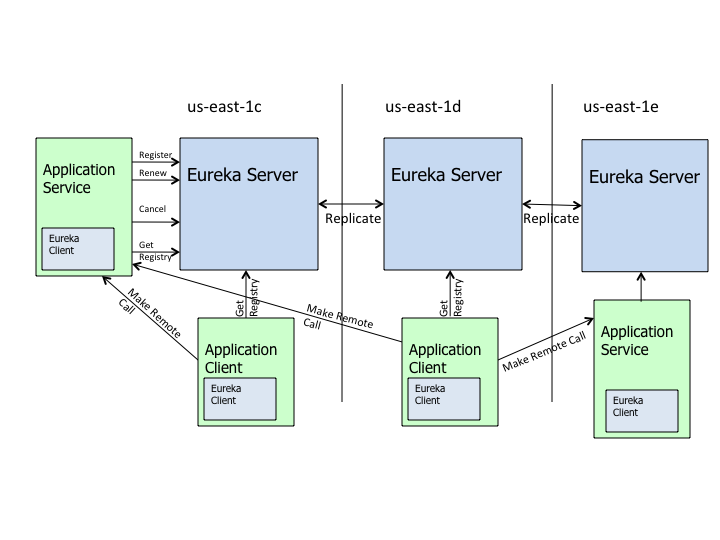
\includegraphics[width=\textwidth, trim={0 4cm 0 0}]{images/netflixEureka/eureka_architecture.png}
    \caption{przykładowa architektura klastra usług Eureka w Netflixie\cite{netflixEurekaGithub}}
    \label{fig:enter-label}
\end{figure}

Powyższa architektura przedstawia sposób, w jaki Eureka jest wdrażana w Netflixie i jest to typowy sposób jej uruchamiania. Na każdy region przypada jedna usługa (bądź też klaster usług) Eureka, w którym rejestrują się instancje z tego regionu, w którym jest uruchomiona. Usługi rejestrują się w serwerze Eureka, a następnie co 30 sekund wysyłają wiadomość hearbeat (\english{heartbeats}), aby odnowić swoje dzierżawy. Jeżeli usługa nie może odnowić dzierżawy kilka razy, jest ona usuwana z rejestru serwera w ciągu około 90 sekund. Informacje o rejestracji i odnowieniach są replikowane na wszystkich węzłach Eureka w klastrze. Klienci z dowolnej strefy mogą wyszukiwać informacje w rejestrze, aby zlokalizować swoje usługi (które mogą znajdować się w innej strefie niż klient) następnie po otrzymaniu informacji o szukanej instancji, klient wykonuje połączenie do usługi\cite{netflixEurekaArticleWang}\cite{netflixEurekaGithub}\cite{springEureka}\cite{netflixEurekaManual}.

\section{Docker}

\begin{figure}[!htbp]
    \centering
    
\includegraphics[width=0.2\textwidth]{images/Docker_logo.png}
    \caption{Logo marki Docker \cite{DockerMedia}}
    \label{fig:enter-label}
\end{figure}

W przeszłości aplikacje były zazwyczaj wdrażane na serwerach fizycznych lub maszynach wirtualnych. Przed wdrożeniem aplikacji należy skonfigurować niezbędną infrastrukturę. Obejmowało to instancję systemu operacyjnego, wszelkich zależności wymaganych przez aplikację i skonfigurowanie wszystkiego by ze sobą współpracowało w prawidłowy sposób. Było to czasochłonne i skomplikowane, zwłaszcza gdy próbowało się odtworzyć dokładnie to środowisko, dla którego aplikacja została stworzona.
Maszyny wirtualne stanowią pod tym względem znaczącą przewagę nad serwerami fizycznymi. Umożliwiają one programistom oddzielenie tworzonego oprogramowania od bazowego systemu. Dodatkowo, oferują one deweloperom łatwo dostępne środowisko, które mogli wykorzystywać do rozwoju i testowania, oddzielone od głównego systemu operacyjnego. Jednak maszyny wirtualne także posiadają swój własny zestaw wyzwań\cite{dockerContenerizationKeyAndUseCases}. 

Jednym z głównych problemów jest to, że wymagają one pełnej kopii systemu operacyjnego. Oznacza to, że są one stosunkowo duże i zajmują dużo zasobów. Z tego powodu uruchamianie wielu maszyn wirtualnych na tym samym serwerze fizycznym jest stosunkowo kosztowne. Nie tylko uruchomienie setek maszyn wirtualnych jest kosztowne, ale także wymaga dużej ilości zasobów, takich jak rdzenie procesora, pamięć \acronym{RAM} (\english{Random Access Memory}) i przestrzeń dyskowa. Co więcej, trudno jest skalować aplikacje w poziomie, co oznacza konieczność dodania większej liczby replik aplikacji w celu obsłużenia zwiększonego ruchu, liczby użytkowników, czy obciążenia pracy danej repliki \cite{dockerContenerizationKeyAndUseCases}.

Konteneryzacja oferuje natomiast szereg korzyści, które pozwalają sprostać tym wyzwaniom. Dzięki konteneryzacji, deweloperzy mogą spakować swoje aplikacje i ich zależności w jednym kontenerze. Obraz Kontenera można natomiast dostarczyć i wdrożyć na dowolnej platformie, która go obsługuje. Ułatwia to wdrożenie i uruchamianie aplikacji w rożnych środowiskach. Konteneryzacja oferuje spójne i niezawodne działanie aplikacji na różnych platformach, niezależnie od tego czy jest to serwer fizyczny, maszyna wirtualna w chmurze, czy też system operacyjny Windows lub Linux\cite{dockerContenerizationKeyAndUseCases}\cite{dockerOverview}. 

Dodatkowymi atutami konteneryzacji są:

\begin{itemize}
    \item \textbf{Przenośność}: Skonteneryzowane aplikacji może łatwo przenieść między różnymi środowiskami. Na przykład, można je łatwo przenieść z laptopa dewelopera do środowiska przejściowego lub produkcyjnego. Nie trzeba martwić się o różne konfiguracje między laptopem a serwerem, na którym zostanie wdrożony kontener\cite{dockerContenerizationKeyAndUseCases}\cite{dockerOverview}.
    
    \item \textbf{Izolacja}: Kontenery zapewniają warstwę izolacji między aplikacją a systemem hosta. Jest to coś w rodzaju bariery ochronnej, która pomaga zapobiegać konfliktom między różnymi aplikacjami lub zależnościami. Każdy kontener działa w swoim własnym, odizolowanym środowisku. Oznacza to, że jest mniej prawdopodobne, że wpłyną na niego inne aplikacje lub procesy działające na tej samej maszynie hosta. W związku z tym znacznie trudniej jest aplikacjom w kontenerach negatywnie wpływać na siebie nawzajem lub na system hosta. Pliki w systemie hosta i w innych kontenerach pozostaną nienaruszone, ponieważ aplikacja nie może uzyskać dostępu do plików spoza własnego środowiska\cite{dockerContenerizationKeyAndUseCases}\cite{dockerOverview}.

    \item \textbf{Wydajność zasobów}: Kontenery umożliwiają uruchamianie wielu odizolowanych aplikacji w tym samym systemie hosta. Nie trzeba przydzielać zasobów do każdej z nich z osobna (jak ma to miejsce w przypadku maszyn wirtualnych). Skutkuje to znacznym zmniejszeniem wykorzystania zasobów i kosztów. Ta zaleta jest szczególnie korzystna w środowiskach chmurowych, gdzie opłaty są często oparte na wykorzystaniu zasobów\cite{dockerContenerizationKeyAndUseCases}\cite{dockerOverview}.

    \item \textbf{Łatwe pakowanie, dostarczanie i wdrażanie}: Dla dewelopera spakowanie aplikacji do obrazu kontenera jest prostym procesem. Następnie deweloper może przesłać zbudowany obraz do rejestru kontenerów, który działa jako scentralizowany serwer do dystrybucji obrazu innym osobom. W ten sposób inne osoby mogą w prosty sposób pobrać zbudowany obraz na swoje urządzenie i go uruchomić\cite{dockerContenerizationKeyAndUseCases}\cite{dockerOverview}.
\end{itemize}

W 2013 roku powstało narzędzie Docker, które znacząco ułatwiło pracę z wykorzystaniem kontenerów. Z wykorzystaniem tego narzędzia można było tworzyć obrazy, przesyłać je do repozytorium, uruchamiać kontenery, łączyć je w sieci i wykonywać wiele innych zadań związanych z kontenerami. Oznacza to, że wystarczy użyć tylko jednego narzędzia aby obsłużyć wszystkie potrzeby związane z kontenerami. W rezultacie kontenery stały się głównym nurtem i zyskały ogromną popularność\cite{dockerContenerizationKeyAndUseCases}\cite{dockerOverview}.

\subsubsection{Docker Compose}

Docker Compose to narzędzie do definiowania i uruchamiania aplikacji wielokontenerowych. Jest to klucz do odblokowania usprawnionego i wydajnego środowiska programowania i wdrażania.
Docker Compose upraszcza kontrolę nad całym stosem aplikacji, ułatwiając zarządzanie usługami, sieciami i wolumenami w jednym, zrozumiałym pliku konfiguracyjnym \akronim{YAML} (\english{YAML Ain’t Markup Language}). Następnie za pomocą jednego polecenia można utworzyć i uruchomić wszystkie usługi z pliku konfiguracyjnego. Compose działa we wszystkich środowiskach: produkcyjnym, przejściowym, deweloperskim, testowym, a także w przepływach pracy \akronim{CI} (\english{Continuous Integration})\cite{dockerComposeAStudyMultiContainerSystem}\cite{dockerComposeOverview}\cite{dockerComposePaterns}.

Docker Compose posiada również polecenia do zarządzania całym cyklem życia aplikacji: 
\begin{itemize}
    \item Uruchamianie, zatrzymywanie i przebudowywanie stosu usług
    \item Wyświetlenie stanu uruchomionych aplikacji
    \item Przesyłanie strumieniowe danych wyjściowych dziennika uruchomionych usług
    \item Uruchamianie jednorazowego polecenia w określonym kontenerze
\end{itemize}

\section{Elasticsearch}

\begin{figure}[!htbp]
    \centering
    \includesvg[width=0.1\textwidth]{images/ELK-Stack/logo-elasticsearch-32-color.svg}
    \caption{Logo Elasticsearch \cite{elasticSearchManualDataIn}}
    \label{fig:enter-label}
\end{figure}

Elasticsearch to rozproszony magazyn dokumentów. Zamiast przechowywać informacje w postaci encji, Elasticsearch przechowuje złożone struktury danych, które zostały serializowane jako dokumenty \akronim{JSON} (\english{JavaScript Object Notation}). W przypadku posiadania wielu węzłów Elasticsearch w klastrze, przechowywane dokumenty są dystrybuowane w całym klastrze i można uzyskać do nich natychmiastowy dostęp z dowolnego węzła\cite{elasticSearchManualDataIn}. 

Elasticsearch jest zbudowany tak, aby był zawsze dostępny i skalował się zgodnie z wymaganiami systemu w którym pracuje. Osiąga to dzięki swojej rozproszonej naturze. Dodając węzły do klastra zwiększa się jego pojemność a następnie Elasticsearch automatycznie rozdzieli dane i obciążenie na wszystkie dostępne węzły. Nie ma potrzeby przebudowywania aplikacji, Elasticsearch sam zrównoważy klastry wielowęzłowe, aby zapewnić wysoką dostępność.

Gdy dokument jest przechowywany w systemie, jest indeksowany i w pełni przeszukiwalny. Elasticsearch wykorzystuje strukturę danych zwaną odwróconym indeksem, który obsługuje bardzo szybkie wyszukiwanie pełnotekstowe. Odwrócony indeks wyszczególnia każde unikalne słowo, które pojawia się w dowolnym dokumencie i identyfikuje wszystkie dokumenty, w których każde słowo występuje\cite{elasticSearchManualDataIn}.  

Indeks można traktować jako zoptymalizowaną kolekcję dokumentów, a każdy dokument jest zbiorem pól, które są parami klucz--wartość zawierającymi dane. Domyślnie Elasticsearch indeksuje wszystkie dane w każdym polu, a każde indeksowane pole ma dedykowaną, zoptymalizowaną strukturę danych.
Na przykład pola tekstowe są przechowywane w indeksach odwróconych, a pola numeryczne i geograficzne są przechowywane w drzewach \akronim{BKD}. Zdolność do korzystania ze struktur danych dla poszczególnych typów pól do gromadzenia i zwracania wyników wyszukiwania sprawia, że Elasticsearch jest w stanie szybko przetwarzać dane\cite{elasticSearchManualDataIn}.

Elasticsearch ma również możliwość nieposiadania, z góry predefiniowanego schematu, co oznacza że dokumenty mogą być indeksowane bez wyraźnego określenia sposobu obsługi każdego z pól, które mogą wystąpić w dokumencie. Gdy dynamiczne mapowanie jest włączone, Elasticsearch automatycznie wykrywa i dodaje nowa pola do indeksu. To domyślne zachowanie ułatwia indeksowanie i eksplorację danych, w momencie indeksowania, Elasticsearch wykrywa i mapuje wartości logiczne, zmiennoprzecinkowe, całkowite, daty i ciągi znaków na odpowiednie typy danych\cite{elasticSearchManualDataIn}. 

Ostatecznie jednak użytkownik wie więcej o swoich danych i sposobie ich wykorzystania niż Elasticsearch. Użytkownik może zdefiniować reguły kontrolujące dynamiczne mapowanie i jawnie zdefiniować konwersję, aby przejąć pełną kontrolę nad sposobem przechowywania i indeksowania pól\cite{elasticSearchManualDataIn}.

Definiowanie własnych mapowań umożliwia:

\begin{itemize}
    \item Rozróżnianie pełnotekstowych pól łańcuchowych i pól łańcuchowych z dokładną wartością.
    \item Przeprowadzanie analizy tekstu specyficznej dla języka
    Optymalizację pól pod kątem częściowego dopasowywania
    \item Używanie niestandardowych formatów daty
    \item Używanie typów danych, takich jak \verb|geo_point| i \verb|geo_shape|, których nie można wykryć automatycznie.
\end{itemize}

Często przydatne jest indeksowanie tego samego pola na różne sposoby w różnych celach. Na przykład, użytkownik może chcieć indeksować pole łańcuchowe zarówno jako pole tekstowe do wyszukiwania pełnotekstowego, oraz jako pole słów kluczowych do sortowania lub agregowania danych. Można też użyć więcej niż jednego analizatora języka do przetworzenia zawartości pola łańcuchowego zawierającego dane wejściowe użytkownika\cite{elasticSearchManualDataIn}.

\section{Logstash}

\begin{figure}[!htbp]
    \centering
    \includesvg[width=0.1\textwidth]{images/ELK-Stack/logo-logstash-32-color.svg}
    \caption{Logstash logo\cite{logstashMain}}
    \label{fig:enter-label}
\end{figure}

Logstash to silnik gromadzenia danych typu otwarto źródłowego (\english{Open source}) z możliwością potokowania w czasie rzeczywistym. Logstash może dynamicznie ujednolicić dane z różnych śródeł i normalizować je do wybranych miejsc docelowych. Oczyszcza i demokratyzuje wszystkie dane dla różnorodnych zaawansowanych zastosować analiztycznych i wizualizacyjnych\cite{logstashManualIntroduction}.

Logstash pierwotnie napędzał innowacje w zakresie gromadzenia logów, jego możliwości wykraczają dlatego poza ten przypadek użycia. Każdy rodzaj zdarzenia można wzbogacić i przekształcić za pomocą szerokiej gamy wtyczek wejściowych, filtrujących i wyjściowych, a wiele natywnych kodeków dodatkowo upraszcza proces pozyskiwania danych. Logstash przyspiesza pozyskiwanie informacji poprzez wykorzystanie większej ilości i różnorodności danych\cite{logstashManualIntroduction}.

Potok przetwarzania zdarzeń Logstash składa się z trzech etapów:

\begin{figure}[!htbp]
    \centering
    \includesvg[width=0.15\textwidth]{schemas/logstashPipeline.drawio.svg}
    \caption{Przetwarzanie zdarzeń w logstash}
    \label{fig:enter-label}
\end{figure}

Wejścia generują zdarzenia, następnie są one filtrowane aby ostatecznie wyjścia wysłały je do miejsca docelowego. Wejścia i wyjścia obsługują kodeki, które umożliwiają kodowanie lub dekodowanie danych wchodzących lub wychodzących z potoku bez konieczności  stosowania oddzielnego filtra\cite{logstashManualHowItWorks}. 

\subsubsection{Wejścia}

Wejścia służą do pobierania danych do Logstash. Niektóre z najczęściej używanych wejść to:

\begin{itemize}
    \item file: odczyt z pliku w systemie plików, podobnie jak w polecenie w UNIX \termdef{tail -0F}\cite{logstashManualHowItWorks}.
    \item syslog: nasłuchuje na porcie 514 i analizuje je zgodnie z formatem RFC3164\cite{rfc3164}\cite{logstashManualHowItWorks}.
    \item redis: oczytuje z serwera redis, używając zarówno kawałków oraz list. Redis jest często używany jako "broker" w scentralizowanym systemie. Logstash, który kolejkuje zdarzenia od zdalnych nadawców\cite{logstashManualHowItWorks}.
    \item beats: przetwarza zdarzenia wysłane przez Beats\cite{logstashManualHowItWorks}.
\end{itemize}

\subsubsection{Filtry}

Filtry są pośrednimi urządzeniami przetwarzającymi w potoku. Filtry można łączyć z instrukcjami warunkowymi w ceu wykonania akcji na zdarzeniu, jeśli spełnia ono określone kryteria. Niektóre przydatne filtry obejmują: 

\begin{itemize}
    \item \textbf{grok}: parsuje i strumieniuje dowolny tekst. Grok jest obecnie najlepszym sposobem w Logstash na analizowanie nieustrukturyzowanych danych dziennika w celu przetworzenia danych w formę nadającą się do zapytań\cite{logstashManualHowItWorks}. 
    \item \textbf{mutate}: wykonuje ogólne transformacje na polach zdarzeń. Można edytować nazwy, usuwać, zastępować i modyfikować pola w zdarzeniach.
    \item \textbf{drop}: pozwala na całkowicie odrzucenie zdarzenia\cite{logstashManualHowItWorks}.
    \item \textbf{clone}: tworzy kopię zapasową zdarzenia, ewentualnie dodając lub usuwając pola\cite{logstashManualHowItWorks}.
    \item \textbf{geoip}: dodawanie informacji o położeniu geograficznym adresów IP\cite{logstashManualHowItWorks}.
\end{itemize}

\subsubsection{Wyjścia}

Wyjścia są ostatnią fazą potoku Logstash. Zdarzenie może przechodzić przez wiele wyjść, ale po zakończeniu przetwarzania wszystkich danych wyjściowych zdarzenie kończy swoje wykonanie\cite{logstashManualHowItWorks}.
Niektóre często używane wyjścia obejmują:

\begin{itemize}
    \item \textbf{elasticsearch}: wysyła dane zdarzeń do Elasticsearch\cite{logstashManualHowItWorks}.
    \item \textbf{file}: zapisywanie danych zdarzeń do pliku na dysku\cite{logstashManualHowItWorks}.
    \item \textbf{graphite}: wysyła dane do zdarzeń do graphite, popularnego otwarto źródłowego narzędzia do przechowywania i tworzenia wykresów metryk\cite{logstashManualHowItWorks}.
\end{itemize}

\subsubsection{Kodeki}

Kodeki to filtry strumieniowe, które mogą działać jako część wejścia lub wyjścia. Kodeki umożliwiają łatwe oddzielenie transportu wiadomości od procesu serializacji. Do najpopularniejszych kodeków należą:

\begin{itemize}
    \item \textbf{json}: koduje lub dekoduje dane w formacie JSON\cite{logstashManualHowItWorks}.
    \item \textbf{multiline}: łączy wielowierszowe zdarzenia tekstowe, takie jak wyjątki w javia i komunikaty zrzutem stosu (\english{Stack trace}) w jedno zdarzenie\cite{logstashManualHowItWorks}.
\end{itemize}

\section{Metricbeat}


\begin{figure}[!htbp]
    \centering
    \includesvg[width=0.1\textwidth]{images/ELK-Stack/icon-metricbeat-32-color.svg}
    \caption{Logo Metricbeat\cite{metricbeatLogo}}
    \label{fig:enter-label}
\end{figure}

Metricbeat to program wykorzystywany do okresowego zbierania metryk z systemu operacyjnego i usług działających na serwerze. Metricbeat pobiera zebrane metryki i statystyki a następnie wysyła je do okreslonych przez użytkownika punktów docelowych, takich jak Elasticsearch, Logstash, Redis lub Kafka\cite{metricbeatOverview}.


\section{Kibana}

\begin{figure}[!htbp]
    \centering
    \includesvg[width=0.1\textwidth]{images/ELK-Stack/logo-kibana-32-color.svg}
    \caption{Logo Kibana\cite{kibanaLogo}}
    \label{fig:enter-label}
\end{figure}

Kibana jest to narzędzie do wizualizacji i eksploracji danych wykorzystywane do analizy dokumentów, przechowywanych w stosie oprogramowania Elastic. Kibana umożliwia nadanie kształtu danym oraz poruszanie się po stosie oprogramowania Elastic\cite{kibanaOverview}. 

Kibana między innymi zapewnia następujące funkcjonalności:

\begin{itemize}
    \item \textbf{Wyszukiwanie, obserwowanie i chronienie danych}: Odkrywanie dokumentów,  analizowanie dzienników oraz znajdowanie luk w zabezpieczeniach\cite{kibanaOverview}.
    \item \textbf{Analiza danych}: Wyszukiwanie zależności, wizualizacja danych na grafach, diagramach, mapach oraz tworzenie, pulpitów nawigacyjnych\cite{kibanaOverview}.
    \item \textbf{Monitoring}: Kibana zapewnia możliwość monitorowania całego klastra oprogramowania Elastic oraz kontrolowania dostępu użytkowników do poszczególnych funkcjonalności\cite{kibanaOverview}.
\end{itemize}

\section{Logstash Logback Encoder}

Logstash Logback Encoder to biblioteka zaprojektowana w celu ułatwienia rejestrowania dzienników aplikacji w formacie JSON przy użyciu biblioteki Logback. Koder ten umożliwia ustrukturyzowanie przechowywanie zdarzeń w formacie JSON, ułatwiając analizowanie dzienników przy wykorzystaniu takich narzędzi jak Logstash i Elasticsearch\cite{logstashLogbackEncoderOverview}. 

Kluczowe cechy:

\begin{itemize}
    \item \textbf{Kodowanie JSON}: Podstawową funkcją tego kodera jest kodowanie zdarzeń Logback do formatu JSON\cite{logstashLogbackEncoderOverview}.
    \item \textbf{Konfigurowalny wygląd}: Biblioteka pozwala na dostosowanie układów logów, umożliwiając użytkownikom zdefiniowanie własnej struktury zdarzeń\cite{logstashLogbackEncoderOverview}.
    \item \textbf{Zaawansowane dodatki}: Dodatkowe appendery, takie jak LogstashTcpSocketAppender i AsyncDisruptorAppender, które ułatwiają wysyłanie logów przez sieć lub ich asynchroniczną obsługę\cite{logstashLogbackEncoderOverview}.
    \item \textbf{Wsparcie dla filtrów Logback}: Biblioteka obsługuje filtry Logback, umożliwiając warunkowe logowanie w oparciu o niestandardowe kryteria\cite{logstashLogbackEncoderOverview}.
    \item \textbf{Maskowanie i zmiana}: Wrażliwe informacje w dziennikach mogą być maskowane lub zmieniane w celu zapewnienia zgodności z przepisami dotyczącymi prywatności danych\cite{logstashLogbackEncoderOverview}.
\end{itemize}

Biblioteka jest szczególnie wykorzystywana w systemach rozproszonych do centralizacji dzienników aplikacyjnych z wielu źródeł i usprawniania ich analizy za pomocą narzędzi takich jak stos \akronim{ELK} (Elasticsearch, Logstash, Kibana)\cite{logstashLogbackEncoderOverview}.

Aby zintegrować Logstash Logback Encoder z projektem Java, należy uwzględnić go jako zależność w konfiguracji kompilacji w pliku konfiugracyjnym, dodatkowo należy skonfigurować plik \textit{logback-spring.xml}, tak aby biblioteka korzystała z prawidłowych appenderów\cite{logstashLogbackEncoderOverview}.
\chapter{Monitoring}

\chapter{Kierunki rozwoju}

\chapter{Podsumowanie}



%--------------------------------------
% Literatura
%--------------------------------------

\bibliographystyle{IEEEtran}{\raggedright\sloppy\small\bibliography{bibliografia}}

%--------------------------------------
% Spis ilustracji
%--------------------------------------
\newpage
\listoffigures

%--------------------------------------
% Spis listingów
%--------------------------------------
\newpage
\lstlistoflistings

%--------------------------------------
% Dodatki
%--------------------------------------

\cleardoublepage\appendix%

%-------------------------------------
% Informacja o prawach autorskich
%--------------------------------------

\ppcolophon

\end{document}
